\section{Implementation}
In this chapter, we will present how we implemented the features that were necessary for fulfilling each requirement described in the Concept chapter. This will be guided by the code of our current implementation.

\subsection{Choosing technology as a basis}

There are multiple libraries available that provide tool kits for creating interactive maps. In this section, we want to showcase these different libraries and explain on what library interactive floorplan will be built upon. Furthermore, we want to clarify what format of geospatial data will be used in this floorplan.

\subsubsection{Google Maps}
\label{Google Maps}

In March 2011, Google introduced the first indoor floorplans on their map. The intention was to increase the overview in public areas like train stations, malls, and airports.
Users can upload own floorplans (valid formats include for example PNG, PDF or JPEG) to the map, with restriction to only publicly available areas.

Google Maps also offers a very popular API for their services. This allows the integration of Google Maps Services on your website. The usage is free for commercial use up until 28000 calls per day\footnote{According to \url{https://cloud.google.com/maps-platform/pricing/sheet/?hl=de}} and requires an API key.
The Maps JavaScript API comes with direct support for importing GeoJSON and can be customized with own content. It's designed to load maps quickly and is optimized for mobile use. Aside from that it also offers a versatile visualization library, which also includes a Heatmap Layer that helps with visualizing a heatmap (Figure~\ref{fig:GoogleMapsHeatmap}).

\begin{figure}[!hb]
    \centering
    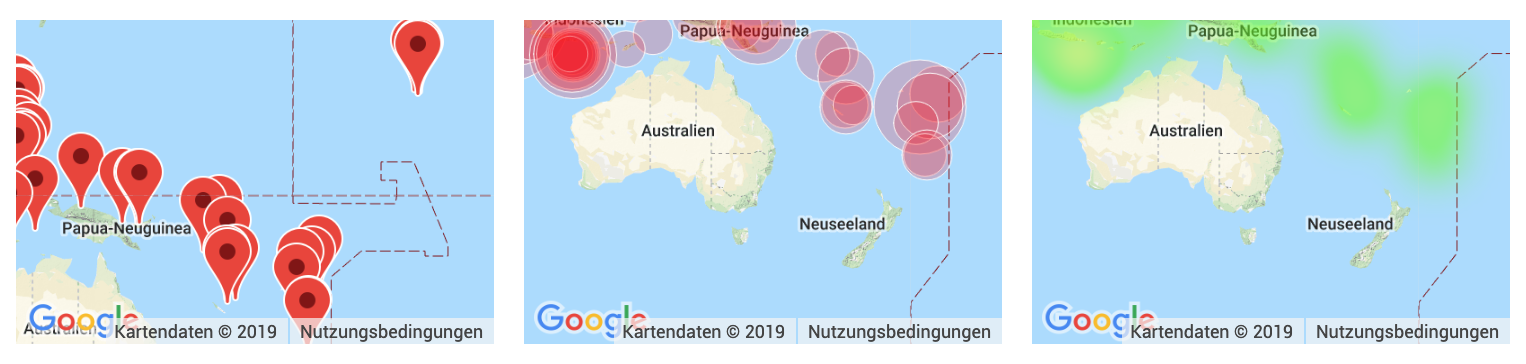
\includegraphics[width=1\linewidth]{images/GoogleMapsHeatmap}
    \caption{Example of visualization options in Google Maps}
    \label{fig:GoogleMapsHeatmap}
\end{figure}

\subsubsection{OpenLayers}
\label{OpenLayers}

OpenLayers is an open-source JavaScript library for displaying interactive maps. Out of the box it comes with various features like map rotation, direct mobile support and import of GeoJSON, TopoJSON, KML\footnote{Keyhole Markup Language} or GML\footnote{Geography Markup Language} data \footnote{\url{https://openlayers.org/}}. Unlike Google Maps, OpenLayers is a pure client-side library with no server-side dependencies. 

\subsubsection{Leaflet}
\label{Leaflet}

Leaflet is another open-source JavaScript library for creating interactive maps. With its first version released in 2011, it is a well established and tested library. 

By only including core features for map visualization, it only has a bundled size of 138.6KB\footnote{\url{https://bundlephobia.com/result?p=leaflet@1.5.1}}, making it a very lightweight library.

Furthermore, Leaflet supports every browser and can easily be extended by plugins from the community or own plugins.
This also includes plugins for creating indoor maps \cite{baines_provides_2019} and real-time maps with Socket.IO.

\subsubsection{GeoJSON}
\label{GeoJSON}

GeoJSON is a format for interchanging geospatial data and is based on JavaScript Object Notation. With the publishing of RFC 7946 in August 2016 it has a standardized format specification.
Different geometries can be represented in a GeoJSON file. These include for example Lines, Linestrings, Polygones or Multipolygones\footnote{\url{https://tools.ietf.org/html/rfc7946}}. 

This can be used to encode the geometry for countries, houses and streets on a map, but also for encoding data for indoor rooms, stairs, and hallways.

\subsubsection{Summary}

Although Google Maps looks very promising for creating our indoor floorplan, there are quite a few problems for us: Because the API needs an internet connection, offline development is not possible. 
Furthermore, the Google Maps API would request payment after hitting the threshold of API calls mentioned above and therefore needs to be linked to an account where billing is activated. Although hitting this threshold could only happen in production, our project partner set the requirement to only use free and also open-source software and linking a billing account of our partner to use the API was not possible. 

Unlike Google Maps, OpenLayers provides an open-source library, which provides a lot of features for interactive maps out of the box.
But because it has a lot of features already bundled together the OpenLayers module is a heavyweight module. With a minified bundle size of 330.1 kB (Version 5.3.3) it takes up to 1.6 seconds to download on 3G\footnote{\url{https://bundlephobia.com/result?p=ol@5.3.3}}. Although this can be lowered for production by deleting unused modules, it takes extra effort to see which modules are not used.

Leaflet solves this problem by providing only a core set of functionalities that can easily be extended by self-written or community plugins. This reduces the size of the module. All in all, we decided to build our interactive map with the Leaflet library, because of its leightweightness and its extensibility, which is useful for configuring the interactive floorplan exactly for our needs. Besides that, we will also use GeoJSON as the format for the external input of the geometric data of each room in the office. We base this decision on the fact that GeoJSON is a widely used and standardized format for encoding geospatial data.

\subsection{Display of indoor features}
\label{Display of indoor features}

The indoor map plugin extends Leaflet by an |Indoor| class, which is able to load in geospatial data from a GeoJSON file (Listing~\ref{listing:setupMapFromGeoJSON}):

\begin{lstlisting}[label={listing:setupMapFromGeoJSON},caption={Setup map from GeoJSON data}]
...
// leaflet map gets rendered inside a div that has the id of the first parameter
this.map = L.map('floorplan-container', {
    center: new L.LatLng(49.41873, 8.67689),
    zoom: 20,
});

const indoorLayer = new L.Indoor(this.props.geoJSON, {
...
\end{lstlisting}

This creates a layer with the GeoJSON data where each feature is represented as an HTML element.
This indoor layer is then added on top of an instance of the  Leaflet |Map|\cite{leaflet:map} class (Listing~\ref{listing:addIndoorLayerToMap}):

\begin{lstlisting}[label={listing:addIndoorLayerToMap},caption={Adding indoor layer to map}]
indoorLayer.addTo(this.map);
\end{lstlisting}


\subsection{Interactive Floorplan}
\label{Interactive Floorplan}

The floorplan handles mouse clicks on each room that is displayed (Listing~\ref{listing:handlingClicksOnARoom}). If a click event occurs, it adds a new marker at this position, which is then automatically linked with the room where the click occurred.

\begin{lstlisting}[label={listing:handlingClicksOnARoom},caption={Handling clicks on a room}]
handleClickOnRoom = (event) => {
    this.addMarker(
        event.latlng, 
        { gateId: undefined, assignedRoomId: event.target.feature.id }, 
        true);
    };
\end{lstlisting}

To create this connection between the room and the marker, each room represented in the GeoJSON file has to have a unique member attribute \emph{id}.\footnote{This is still following the GeoJSON format specification according to \url{https://geojson.org/geojson-spec.html\#feature-objects}}

After setting the marker it needs to be linked with a gate, which is done by a selection input presenting all available gates. After successfully linking it to a gate the marker gets persisted in our database.

The map is capable of also handling pan events for moving to another location and scroll events for zooming in and out. This functionality is part of the |Map| class from Leaflet.

\subsection{Logging of Gate Events}
\label{Logging of Gate Events}

To support the functionality to log gate events we make use of the Elastic Stack\footnote{https://www.elastic.co/de/products/elastic-stack}.
The Elastic Stack consists of mainly three open-source projects: \emph{Elasticsearch}, \emph{Logstash} and \emph{Kibana}.
Together they form a pipeline that can be used to analyze, search and visualize logs created from different sources. 

The component of the first stage of this pipeline is Logstash, which is responsible for collecting data from different locations and transforming it for the next step. Elasticsearch then indexes these logs and provides a RESTful API for searching. Kibana uses this API from Elasticsearch to provide meaningful visualization of the logs.
Through a smart indexing technology, the Elastic Stack promises a fast response time even for large data sets and is used by companies like Netflix for monitoring security-related logs or Medium for debugging production issues \footnote{\url{https://hackernoon.com/elastic-stack-a-brief-introduction-794bc7ff7d4f}}.

%In our project logs sent from the gates need to be analyzed and visualized to give the facility management team more insights about the access decisions made. These information get also displayed in the floorplan and the heatmap gets calculated based on the gate event logs. 
To ensure a fast display of the access decision data and to also ensure the possibility in the future to search and visualize logs not only from the gates, but from other sources also, we decided to utilize the Elastic Stack.

\subsubsection{Elasticsearch Server}

Since we're working with own custom visualization, we will ignore Kibana for our implementation. And since we're only receiving events from one source - the gates, we can skip the Logstash pipeline step and send event data directly to the Elasticsearch server, which then will be stored in a database and indexed.

Since data of any form can be sent to the Elasticsearch server, it performs an automatic type detection for each property that is sent. This can result in wrong datatypes, causing the server to reject future events because they're not fulfilling the required datatypes\footnote{For example: The first event has a member \emph{id} with the value "1234". The Elasticsearch server will automatically interpret this value as an Integer and set it as a required datatype. If the following event now has an id of "fe123d" (String) the server will not accept this event.}. To prevent this, we first have to create a template for our gate event objects, which strictly declares the datatypes for each property in the event object (Listing~\ref{listing:curlScriptTemplateElastic}):

\clearpage

\begin{lstlisting}[label={listing:curlScriptTemplateElastic},caption={cURL script for creating gates index template}]
curl -v -X PUT 'localhost:9200/_template/gates' -H 'Content-Type: application/json' -d '
{
  "index_patterns" : ["gates"],
  "settings": {
  /* Shards allow to split up the content volume that is taken by the documents that are inside a single index. This enables good scaling, by allowing the documents not to reside on just one single harddrive but multiple. Since we are currently not receiving that much data yet it is sufficient to only work with one shard for now.*/
    "number_of_shards": 1
  },
  "mappings": {
    "_source": {
    // allows for example updating a document
      "enabled": true
    },
    "properties": {
      "timestamp": { "type": "date" },
      "loglevel": { "type": "keyword" },
      "gateId": { "type": "keyword" },
      "deviceId": { "type": "keyword" },
      "accessType": { "type": "keyword" },
      "wasSuccessful": { "type": "boolean"},
      "message": { "type": "text"}}
  }
}'
\end{lstlisting}

%TODO Was ist unterschied zwischen integer und keyword, warum ist die suche dadurch besser?

We then create a \emph{gates} index (Listing~\ref{listing:elasticsearchGatesIndex}). All logs for the gates will be stored under that index.

\begin{lstlisting}[label={listing:elasticsearchGatesIndex},caption={cURL script for creating gates index}]
curl -v -X PUT 'localhost:9200/gates'
\end{lstlisting}

This server then offers an REST API endpoint for creating gate event logs (Listing~\ref{listing:searchElasticPOST}).

 \clearpage
 
\begin{lstlisting}[label={listing:searchElasticPOST},caption={Interface of Elasticsearch server to create gate event logs}]
function postGateEvent(eventData) {
    return fetch(`http://${elasticsearchBasePath}/gates/_doc`, {
        headers: {
            'Content-Type': 'application/json',
        },
        body: eventData,
        method: 'POST',
    })
        .then(response => errorHandling.checkResponseOk(response, msg.getCreateEventFailMsg(response)));
}
\end{lstlisting}

This endpoint is exposed to the outside so gates can communicate to our system. To protect this route from being exploited from other sources than the gates we use a preshared token that needs to be set in the \emph{Authorization} header.
 The endpoint requires a transfer of the ID of the device that tried to access, the access type (entry or exit), the gate ID and if the entry or exit was successful. Moreover, the optional parameters |loglevel| and |message| can be sent. The |loglevel| can be used to signalize an alarm event and the |message| parameter can be used to send over more detailed information.

The Elasticsearch server also offers an interface to search for logs satisfying specific conditions. This is how we can look up all the events at a gate that are of a specific access type (Listing~\ref{listing:elasticsearchRequest}):

\clearpage

\begin{lstlisting}[label={listing:elasticsearchRequest},caption={Example search request to Elasticsearch server}]
function fetchAllEventsAtGateWithAccessType(gateId, accessType) {
    const now = new Date().toISOString();
    const officeOpening = getOfficeOpeningDatetime().toISOString();

    const url = `http://${elasticsearchBasePath}/gates/_search?sort=timestamp:desc&`
        +  `q=gateId:${gateId}`
        +  `%20AND%20`
        +  `accessType=${accessType}`
        +  `%20AND%20`
        +  `timestamp:[${officeOpening}+TO+${now}}`;
        
    return fetch(url, {
        headers: {
            Accept: 'application/json',
        },
    })
        .then(response => errorHandling.checkResponseOk(response));
}
\end{lstlisting}

\subsection{Real-time Floorplan}
\label{Real-time Floorplan}

To implement a real-time floorplan we utilize the \emph{Socket.IO} JavaScript library, a library which enables to implement real-time applications. This is achieved through an event-based, bidirectional communication between the client and the server. 

Although Socket.IO also uses WebSockets for transportation it is not an implementation of the WebSocket-protocol. It extends and combines multiple real-time protocols and switches between them if needed. Therefore a connection can only be established between a Socket.IO client and a Socket.IO server\footnote{\url{https://socket.io/docs/index.html}}.

We decided to use Socket.IO, because of its easy to understand API and its functionality set. It provides the creation of reliable connections by having different fallback real-time methods, auto reconnection support and the detection of disconnections.

In the following sections, we will explain the setup of Socket.IO in the backend and frontend and how this setup is used to implement a real-time floorplan.

\subsubsection{Backend}
\label{Backend}

We first have to create a Socket.IO |Server|\cite{socketio:server} instance by binding it to the existing HTTP server we have for our backend (Listing~\ref{listing:creationOfSocketIOserver}):

\begin{lstlisting}[label={listing:creationOfSocketIOserver},caption={Creation of Socket.IO server}]
//app.js
const server = http.createServer(app);
socketHelpers.handleSockets(server);

//socket.helpers.js
function handleSockets(server) {
    // creates Socket.IO Server
    const io = socketIo(server);
    ...
}
\end{lstlisting}

To ensure that we only send data to clients that are authenticated, we need to verify the token that is sent with each packet. This is done by installing a middleware on to our Socket.IO server that includes a function that gets executed for every packet that is sent. This function verifies that the token sent is a valid access token (Listing~\ref{listing:createSocketIOMiddleware}).

\begin{lstlisting}[label={listing:createSocketIOMiddleware},caption={Middleware of Socket.IO server}]
io.use((socket, next) => {
    const { token } = socket.handshake.query;
    const verifyToken = keycloakHelpers.verifyToken(token);
    return verifyToken
        .then(() => next())
        .catch(err => next(err));
});
\end{lstlisting}

Every time a frontend client now connects to the server, the server extracts the userId from the token that was sent by the client. We then create a \emph{Room}\cite{socketio:rooms} - a separate communication channel - with this userId, so that we can emit notifications only to that specific user. If the logged-in user is also an admin, he gets added to an admin room, a room where all other admins that are connected are also inside. The implementation of this can be seen in Listing~\ref{listing:onConnection}.

\begin{lstlisting}[label={listing:onConnection},caption={Handling client connections to Socket.IO server}]
io.on('connection', (socket) => {
    const { token } = socket.handshake.query;
    const parsedToken = jwt.decode(token);

    const isAdmin = parsedToken.realm_access.roles.includes('admin');
    const userId = parsedToken.sub;

    if (isAdmin) socket.join('admin');
    socket.join(userId);
});
\end{lstlisting}

We can then emit messages to specific users or to all admins through a helper function (Listing~\ref{listing:emitMessage}):
\begin{lstlisting}[label={listing:emitMessage},caption={Helper function for emitting notifications}]
module.exports.emitMessage = (user, emitType, message) => {
    // user can be either a userId or 'admin'
    // all current client sessions with logged in user will receive message
    io.to(user).emit(emitType, message);
};
\end{lstlisting}

This method gets called every time the gates send an event through our backend interface that we presented earlier. We use the room 'admin' to notify all admins at the same time (Listing~\ref{listing:socketIOBackendNotification}).

\begin{lstlisting}[label={listing:socketIOBackendNotification},caption={Emission of notification to all admins}]
function notifyAboutEvent(data) {
    if (data.loglevel.toUpperCase() === constants.ALARM_LOG_LEVEL) {
        notificationHelpers.notifyAdminOnAlarm(data);
    } else {
        socketHelpers.emitMessage('admin', socketHelpers.GATE_EVENT, data);
    }
}
\end{lstlisting}

\subsubsection{Frontend}
\label{Frontend}

The frontend has to install the Socket.IO JavaScript library and then initialize a |Socket|\cite{socketio:socket}. Handlers are then registered to that |Socket| for the different notification events from the backend (Listing~\ref{listing:socketIOClientSide}).

\begin{lstlisting}[label={listing:socketIOClientSide},caption={Setup of Socket.IO socket}]
listenForGateEvents = () => {
        const socket = io({
            secure: true,
            // only use WebSocket as transportation method
            transport: ['websocket'],
            query: {
                token: sessionStorage.getItem('kctoken'),
            },
            jsonp: false,
        });

        socket.on('gateEvent', (event) => { this.gateEventHappened(event); });
        socket.on('gateAlarm', (event) => { this.gateAlarmHappened(event); });
    };
\end{lstlisting}


\subsubsection{Heatmap}

Every time an event occurs the marker that is linked with the gate Id of the event object is searched. Then the room id that is connected with this marker is re-colorized based on the updated number of people that are behind this gate (Listing~\ref{listing:gateEventHappened}).

\clearpage

\begin{lstlisting}[label={listing:gateEventHappened},caption={Handling gate events in frontend}]
gateEventHappened = (event) => {
        const gateMarker = this.findGateMarkerWithId(event.gateId);

        if (gateMarker) {
            this.applyPulseEffectToMarker(gateMarker);

            const { assignedRoomId } = gateMarker.options;
            getNumberOfPeopleForGateWithId(event.gateId)
                .then((data) => {
                    this.updateGateInfoOfCurrentSelectedMarker(gateMarker, data);
                    this.colorizeRoom(assignedRoomId, data.count);
                });
        }
    };
\end{lstlisting}

To calculate the number of people we use an endpoint in our backend that looks at the DateTime of the office opening at the day the request to the endpoint is made. At this time we expect that no people are inside the office. It then counts all entries and exits at the gate with the given id that was successful and after the office opening. By subtracting the exits from the entries we get the number of people that are behind this gate.

This result is then the input for colorizing the room (Listing~\ref{listing:colorizeRoom}):

\begin{lstlisting}[label={listing:colorizeRoom},caption={Function for colorizing a room}]
colorizeRoom = (roomId, numberOfPeople) => {
    let occupancyRate = numberOfPeople / constants.ROOM_PERSON_COUNT_LIMIT;
    if (occupancyRate > 1) occupancyRate = 1;
    if (occupancyRate < 0) occupancyRate = 0;

    const room = this.findRoomWithId(roomId);

    room.setStyle({ fillColor: this.getColorForOccupancyRate(occupancyRate) });
};
\end{lstlisting}

Because we can only work with events from the gates and no indoor positioning technology, we're unable to locate the exact position of single device. Therefore we colorize the entire room evenly.

We follow the common convention in heatmaps of representing the occupancy of a room by using colors on a scale from green to red, with green representing a room with no people inside and with red a room that hit its maximum capacity. The calculation for the color can be seen in Listing~\ref{listing:getColorForOccupancyRate}.

\begin{lstlisting}[label={listing:getColorForOccupancyRate},caption={Function for calculating color based on occupancy}]
getColorForOccupancyRate = (rate) => {
    /*
        input: value from 0 to 1
        returns: a hsl color on a scale from green to red
    */
    const hue = ((1 - rate) * 120).toString(10);
    return ['hsl(', hue, ',100%,50%)'].join('');
};
\end{lstlisting}

\subsubsection{Access Decision Information}

More information about the access decisions gets also displayed in real-time in a table (\emph{Activity Monitor}) below the interactive floorplan (Figure~\ref{fig:FloorplanScreenshot}).

\begin{figure}[!hb]
    \centering
    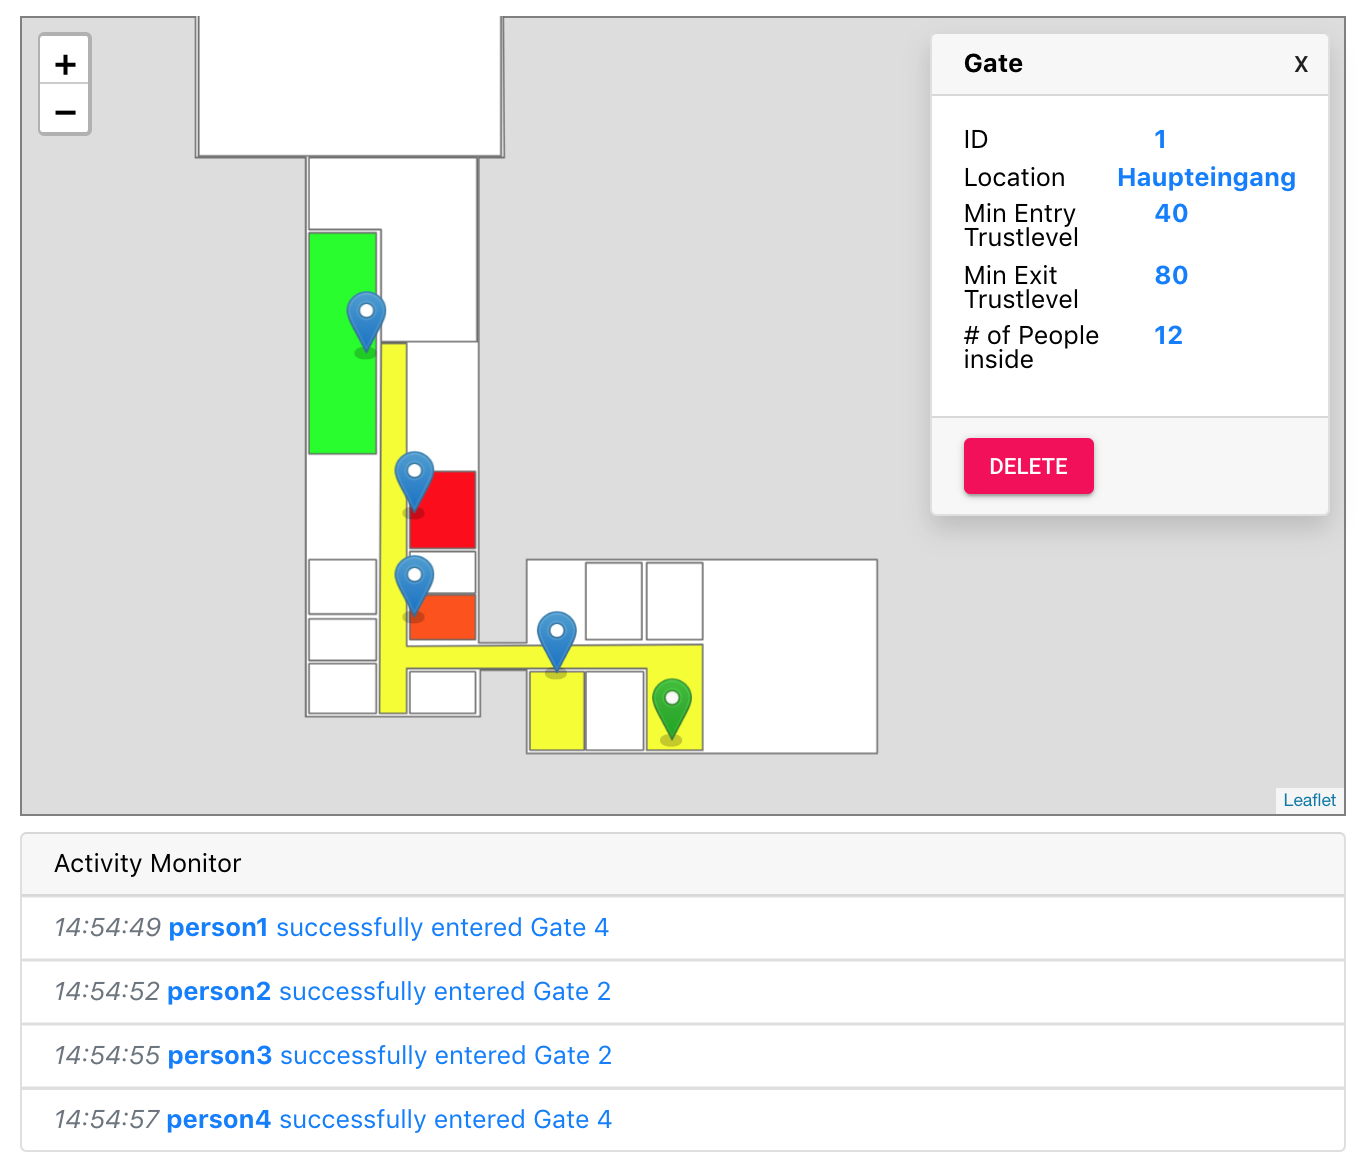
\includegraphics[width=0.9\linewidth]{images/FloorplanScreenshot}
    \caption{Implemented interactive floorplan}
    \label{fig:FloorplanScreenshot}
\end{figure}

Because the gates transmit the deviceId in the event object, the relationship to the owner of the device can be made through our backend. This happens each time a gate event occurs and we add the information as a new row into the Activity Monitor (Listing~\ref{listing:addMessage}):

\begin{lstlisting}[label={listing:addMessage},caption={Function for adding message to Activity Monitor}]
addMessage = (logMessage) => {
        const { logMessages } = this.state;
        
        // only show 100 log messages at a time
        if (logMessages.length >= 100) {
            logMessages.shift();
        }

            // get user information with the device ID provided in the event object
        getDeviceById(logMessage.deviceId)
            .then(device => getUserById(device.userId))
            .then(user => {
                logMessages.push({ ...logMessage, username: user.username});
                this.setState({ logMessages });
                this.scrollToBottom();
            });
    };
\end{lstlisting}

For each event, we display information about the time, the person that is connected with the event, the access type, the success of the access and the gate Id where the event happened.

\subsubsection{Alarm}

To visualize an alarm event at a gate we colorize the marker red and display a red log message in the Activity Monitor (Listing~\ref{listing:alarmEventHappened}):

\begin{lstlisting}[label={listing:alarmEventHappened},caption={Handling gate alarm events in frontend}]
gateAlarmHappened = (event) => {
        const gateMarker = this.findGateMarkerWithId(event.gateId);
        if (gateMarker) {
            this.pulsateMarker(gateMarker, 'red');
        }
    };
\end{lstlisting}

Furthermore the backend automatically sends an email to all admins with the information about the incident (Listing~\ref{listing:notifyOnAlarm}):

\begin{lstlisting}[label={listing:notifyOnAlarm},caption={Notifying admins on alarm event}]
function notifyAdminOnAlarm(alarmEvent) {
    socketHelpers.emitMessage('admin', socketHelpers.GATE_ALARM, alarmEvent);
    // send mail to every admin
    return getMailsOfAdmins()
        .then((mails) => {
            for (const mail of mails) {
                if (mail) mailHelpers.sendAlarmMail(mail, alarmEvent);
            }
        });
}
\end{lstlisting}

\clearpage
